\chapter{行为调节神经回路的计算基础} \label{chap:chap5}

上一章重点介绍了大脑神经解剖学以及大脑不同区域之间的联系。
要了解这些连接是如何调节行为,需要深入了解不同神经元群体活动所代表的信息是如何传递和处理的。
这种理解大部分来自对单个神经元产生的微小电信号的记录。


虽然通过一次记录一个或几个神经元已经了解了很多东西,但小型化和电子技术的进步现在使得同时记录多个大脑区域数百个单个神经元的动作电位成为可能,通常是在感觉、运动或认知任务的背景下(方框~\ref{box:5_1})。这些进步,加上管理和理解大型数据集的计算方法,有望彻底改变我们对神经功能的理解。


\begin{proposition}[光学神经成像] \label{box:5_1}
	
	\quad \quad 光学成像方法是用于大规模监测神经回路动力学的一个快速发展的技术领域。
	这些方法中的大多数都使用荧光传感器(合成染料或基因工程和编码的蛋白质),通过激发后发出的光的大小或波长的变化来发出神经活动变化的信号。
	根据荧光激发的来源,已经开发了各种荧光成像方法,包括单光子、多光子和超分辨率荧光显微成像。
	
	\quad \quad 最常用的荧光指示剂将细胞内钙水平的变化作为神经元电活动的指标。
	虽然荧光钙成像的时间分辨率通常低于电生理学的时间分辨率,但具有基因编码钙指示剂的荧光成像能够在几天到几周和几个月内同时监测行为动物中数千个单独识别的神经元。
	
	\quad \quad 除了钙成像外,合成和遗传编码的电活性荧光指示剂(如\textit{基因编码的电压指示剂})、神经递质浓度报告因子(如\textit{谷氨酸盐感应荧光受体})、细胞内信号分子的活性状态和基因表达为在多个空间和时间尺度上监测神经活动提供了快速扩展和通用的技术。
	
\end{proposition}


与此同时,基于单个神经元\textit{mRNA}测序的现代遗传方法正在揭示促成群体活动的多种细胞类型。
基于遗传的方法还允许在实验期间激活或沉默定义类型的神经元,支持因果关系的测试(方框~\ref{fig:5_2})。


\begin{proposition}[神经元活动的光遗传学和化学遗传学操作] \label{box:5_2}
	
	\quad \quad 神经回路的功能分析依赖于准确操作已识别的回路元件以阐明其在生理和行为中的作用的能力。
	已经开发了基因编码的神经扰动工具,用于使用激活工程受体的光(光遗传学)或小分子(化学遗传学)远程控制神经元功能。
	
	\quad \quad 基因编码的外源蛋白可以使用病毒或转基因动物在分子、基因或空间指定的神经元亚群中表达,用于随后对这些细胞群的选择性扰动。
	光遗传学方法涉及光敏蛋白的表达和随后的光传递到由此产生的光敏神经元。
	根据光遗传学致动器的类型,光激活将分别通过去极化或超极化细胞膜来增强神经活动(例如,通道视紫红质等光控离子通道)或抑制神经活动(如卤视紫红质和古菌视紫红质的光控离子泵)。
	
	\quad \quad 或者,可以使用化学遗传致动器远程激活或沉默选定的神经元群体,化学遗传致动器是使用遗传方法靶向定义的神经元群体的基因工程受体;
	它们可以通过小分子合成配体被激活,该配体在递送时选择性地与这些受体相互作用(例如\textit{设计药物激活的设计受体})。
	
	\quad \quad 这些光遗传学和化学遗传学工具对神经元活动提供了精确的时空控制,以探索神经元细胞类型、回路生理学和行为之间的因果关系。
	
\end{proposition}



在光学显微镜和电子显微镜的尺度上,高通量解剖方法正在以前所未有的详细程度和完整性提供有关回路布线的信息。
神经回路的复杂性和从中收集的大量数据集推动了统计、计算和理论方法的发展和应用,用于提取、分析、建模和解释结果。
这些方法用于研究范围广泛的问题:
实验设计、从原始数据中提取信号、大型复杂数据集的分析、模拟数据的模型的构建和分析,最后也是最重要的是,从结果中建立某种形式的理解。


信号提取通常基于贝叶斯方法进行,推断出嘈杂记录中最有可能出现的信号。
数据分析通常包括减少大型数据集的维数,不仅仅是为了使其更紧凑,而是为了确定构建数据集的基本组件。


神经系统模型的范围从单个神经元的形态学和电生理学的详细模拟到大量神经元的更抽象模型。
无论详细程度如何,模型的目的都是揭示神经元或神经元网络的测量特征如何影响神经元或神经回路的功能。


此外,在最高级别的功能中,例如识别图像、玩游戏或执行人类级别的任务,机器学习的想法正日益影响神经科学研究。


在本章中,我们介绍了用于描述和解释神经群和电路活动的思想、技术和方法,并举例说明了大脑研究的一些领域。本书后面将更详细地讨论其中的许多主题。



\section{神经放电模式提供信息编码}

\subsection{感觉信息由神经活动编码}

动物和人类通过感官不断积累关于世界的信息,根据这些信息做出决定,并在必要时采取行动。
为了处理感官信息以用于决策和行动,必须将其转化为电信号,从而在大脑中产生神经活动模式。
研究这种神经表征及其与外部感觉线索的关系,统称为神经编码,是神经科学研究的一个主要领域。
刺激的特征由神经活动表示的过程称为编码。


神经表征的结构在神经系统如何进一步处理信息方面起着重要作用。
例如,视觉信息最初是在视网膜中通过感光器对一小块视野区域的颜色和光强的反应进行编码的。
然后,这些信息在大脑初级视觉皮层内进行转换,以定义场景的边缘和形状以及这些特征所在的位置为基础,对视觉场景进行编码。
进一步的转换发生在高阶视觉区域,从场景中提取复杂的形状和进一步的结构,包括物体甚至个人面孔的识别。
在大脑的其他区域,听觉编码反映了声音的频谱,触觉编码在代表身体表面的地图中。
神经元对感觉刺激的反应所激发的动作电位序列代表了这种刺激是如何随时间变化的。
神经编码研究旨在了解驱动神经元做出反应的刺激特征和反应的时间结构及其与外部世界变化的关系。



\subsection{可以从神经活动中解码信息}

感觉神经元对感觉特征的反应是通过激发动作电位来编码信息。
其他大脑区域,例如那些导致决策或产生运动动作的区域,必须正确解释它们从感觉区域接收到的动作电位序列的含义,以便做出适当的反应。
从神经活动中提取信息的过程称为解码。


神经信号的解码可以由神经科学家在实验和临床环境中完成。
例如,这种解码可以从视觉或听觉神经元的记录中推断出动物或人类正在看到或听到什么。
在实践中,只有刺激的某些特征可能被推断出来,但结果仍然令人印象深刻。
大量的解码程序已经开发出来,从简单的神经元放电率加权和到复杂的统计方法。


解码方法是神经假体开发的核心,适用于各种神经系统损伤导致大面积瘫痪的人(第~\ref{chap:chap39}~章)。
为了实现这一点,神经元通过植入的电极记录在顶叶皮层或运动皮层中,并使用在线解码程序来解释记录的神经活动所代表的运动意图。
然后使用推断出的意图来控制计算机光标或驱动机器人肢体。


解码记录的神经活动也让我们对神经回路中正在发生的事情有了一个非凡的了解,这反过来又提供了对记忆存储和检索、计划和决策以及其他认知功能。
下一节使用一种特别有趣的神经表征来说明这些见解,即啮齿动物海马体中空间位置的编码。


\subsection{可以解码海马空间认知图来推断位置}

% 定位
动物面临的最复杂的认知挑战之一是识别和记住它在环境中相对于其他显著物体位置的位置。
例如,贮藏种子的鸟类可以记住它们在几个月内储存食物的数百个不同地方的位置。
前一章简要介绍了与外显记忆形成有关的神经回路,即对人、地点、事物和事件的记忆。
这种形式的记忆需要海马体、内嗅皮层和颞叶中的相关结构。
1971 年,\textit{约翰$\cdot$奥基夫}发现了海马体中空间环境的神经表征的生理学证据。
2014 年,他与\textit{梅$\cdot$布里特$\cdot$莫泽}和\textit{爱德华$\cdot$莫泽}一起获得诺贝尔生理学或医学奖,以表彰他们在神经元空间表征方面的发现。


\textit{奥基夫}发现大鼠海马体中的单个细胞(称为位置细胞)仅在动物穿过环境的特定区域(称为细胞位置场)时才会放电(图~\ref{fig:5_1})。
随后的研究发现了其他几种哺乳动物(包括蝙蝠、猴子和人类)海马体中的位置细胞样活动。
不同的位置细胞集由给定环境中的不同位置激活。
因此,虽然单个位置细胞代表相对较小的空间区域,但海马体中完全不同的位置细胞群平铺了整个环境,并且任何给定位置都由独特的细胞群编码。
海马位置编码网络提供了一个认知地图的例子,最初由心理学家\textit{爱德华$\cdot$托尔曼}假设,它使动物能够成功地记住并导航其环境。
第~\ref{chap:chap52}~章和第~\ref{chap:chap54}~章详细探讨了海马体在记忆形成中的作用以及海马体空间图的编码机制。


\begin{figure}[htbp]
	\centering
	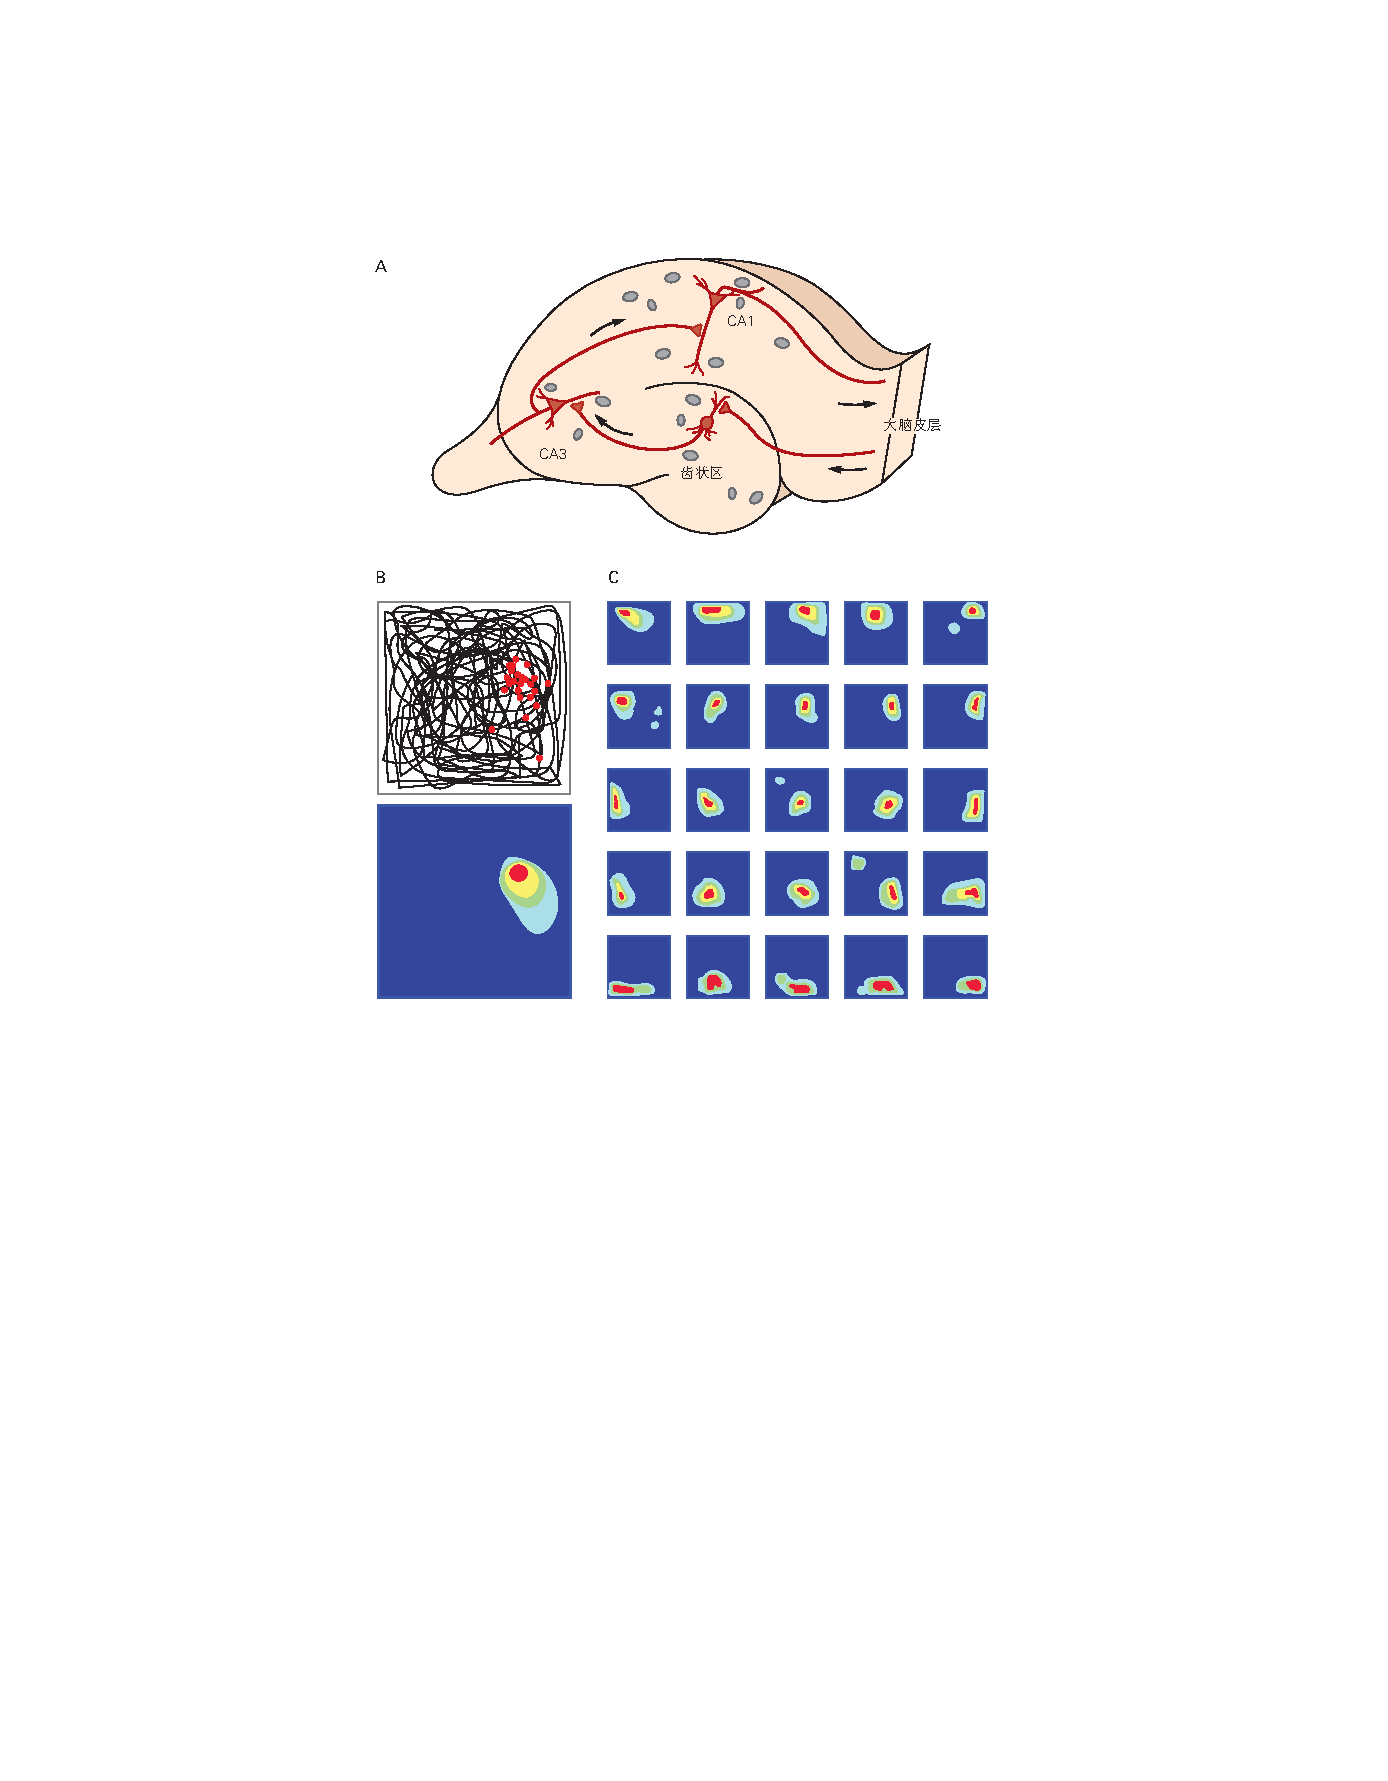
\includegraphics[width=0.9\linewidth]{chap05/fig_5_1}
	\caption{海马体位置细胞和位置细胞图。 
		\textbf{A.} 输入-输出转换发生在哺乳动物海马体的三突触回路中,从\textit{齿状回}输入区到\textit{阿蒙角}3 区,再到\textit{阿蒙角}1 输出区,每个区域的主要兴奋性神经元(红色)作为主要处理单元。
		主要细胞的活动由局部回路\textit{$\gamma$-氨基丁酸}活动的中间神经元(灰色)调节。
		\textbf{B.} 将细胞放电置于海马体中。
		老鼠穿过方形场地时所走的路径以黑色显示。
		电极被植入海马体内以记录单个细胞。
		上图:单个位置细胞会增加环境中离散位置的放电(每个动作电位由一个红点表示)。
		下图:位置细胞激活频率的颜色编码热图。
		较低波长的颜色(黄色和红色)代表在没有活动的背景(深蓝色)下较高的激活率。 
		\textbf{C.} 颜色编码的热图显示当大鼠探索一个方形盒子时在海马\textit{阿蒙角}1 区域同时记录的 25 个不同位置细胞的放电。}
	\label{fig:5_1}
\end{figure}


1971 年\textit{奥基夫}的可用的电生理方法仅限于一次记录一个位置细胞,但随后的进展允许研究人员同时记录数十个,最近数百个位置细胞。
关键的是,虽然单个位置细胞仅对环境的特定部分进行编码,并且容易在其位置场之外偶尔发出嘈杂的信号,但整个位置细胞群提供了更完整的空间覆盖和冗余位置编码的可靠性。
群体编码的这些特征为新的强大的计算分析铺平了道路。
特别是,可以解码位置细胞群体的活动并估计动物在环境中的位置。
这是通过确定每个细胞的空间选择性并使用该选择性作为模板来解码正在进行的活动来实现的。
在实践中,这种解码通常是通过加权每个细胞对动物位置最终估计的贡献来执行的,该因素与该细胞的空间编码可靠性成正比。
使用这种技术和类似技术,人们可以在房间大小的环境中以几厘米的精度逐秒重建动物的位置(图~\ref{fig:5_1}C)。



基于使用空间解码技术的研究,海马体功能与空间和陈述性记忆密切相关。
在积极探索环境期间,海马体活动反映位置编码,但在不动或静止行为期间,海马体进入不同的状态,在该状态下,神经活动由离散的半同步群体爆发主导,称为尖波涟漪(图~\ref{fig:5_2}A))。
这些事件被认为是由海马体内的回路在内部产生的。


\begin{figure}[htbp]
	\centering
	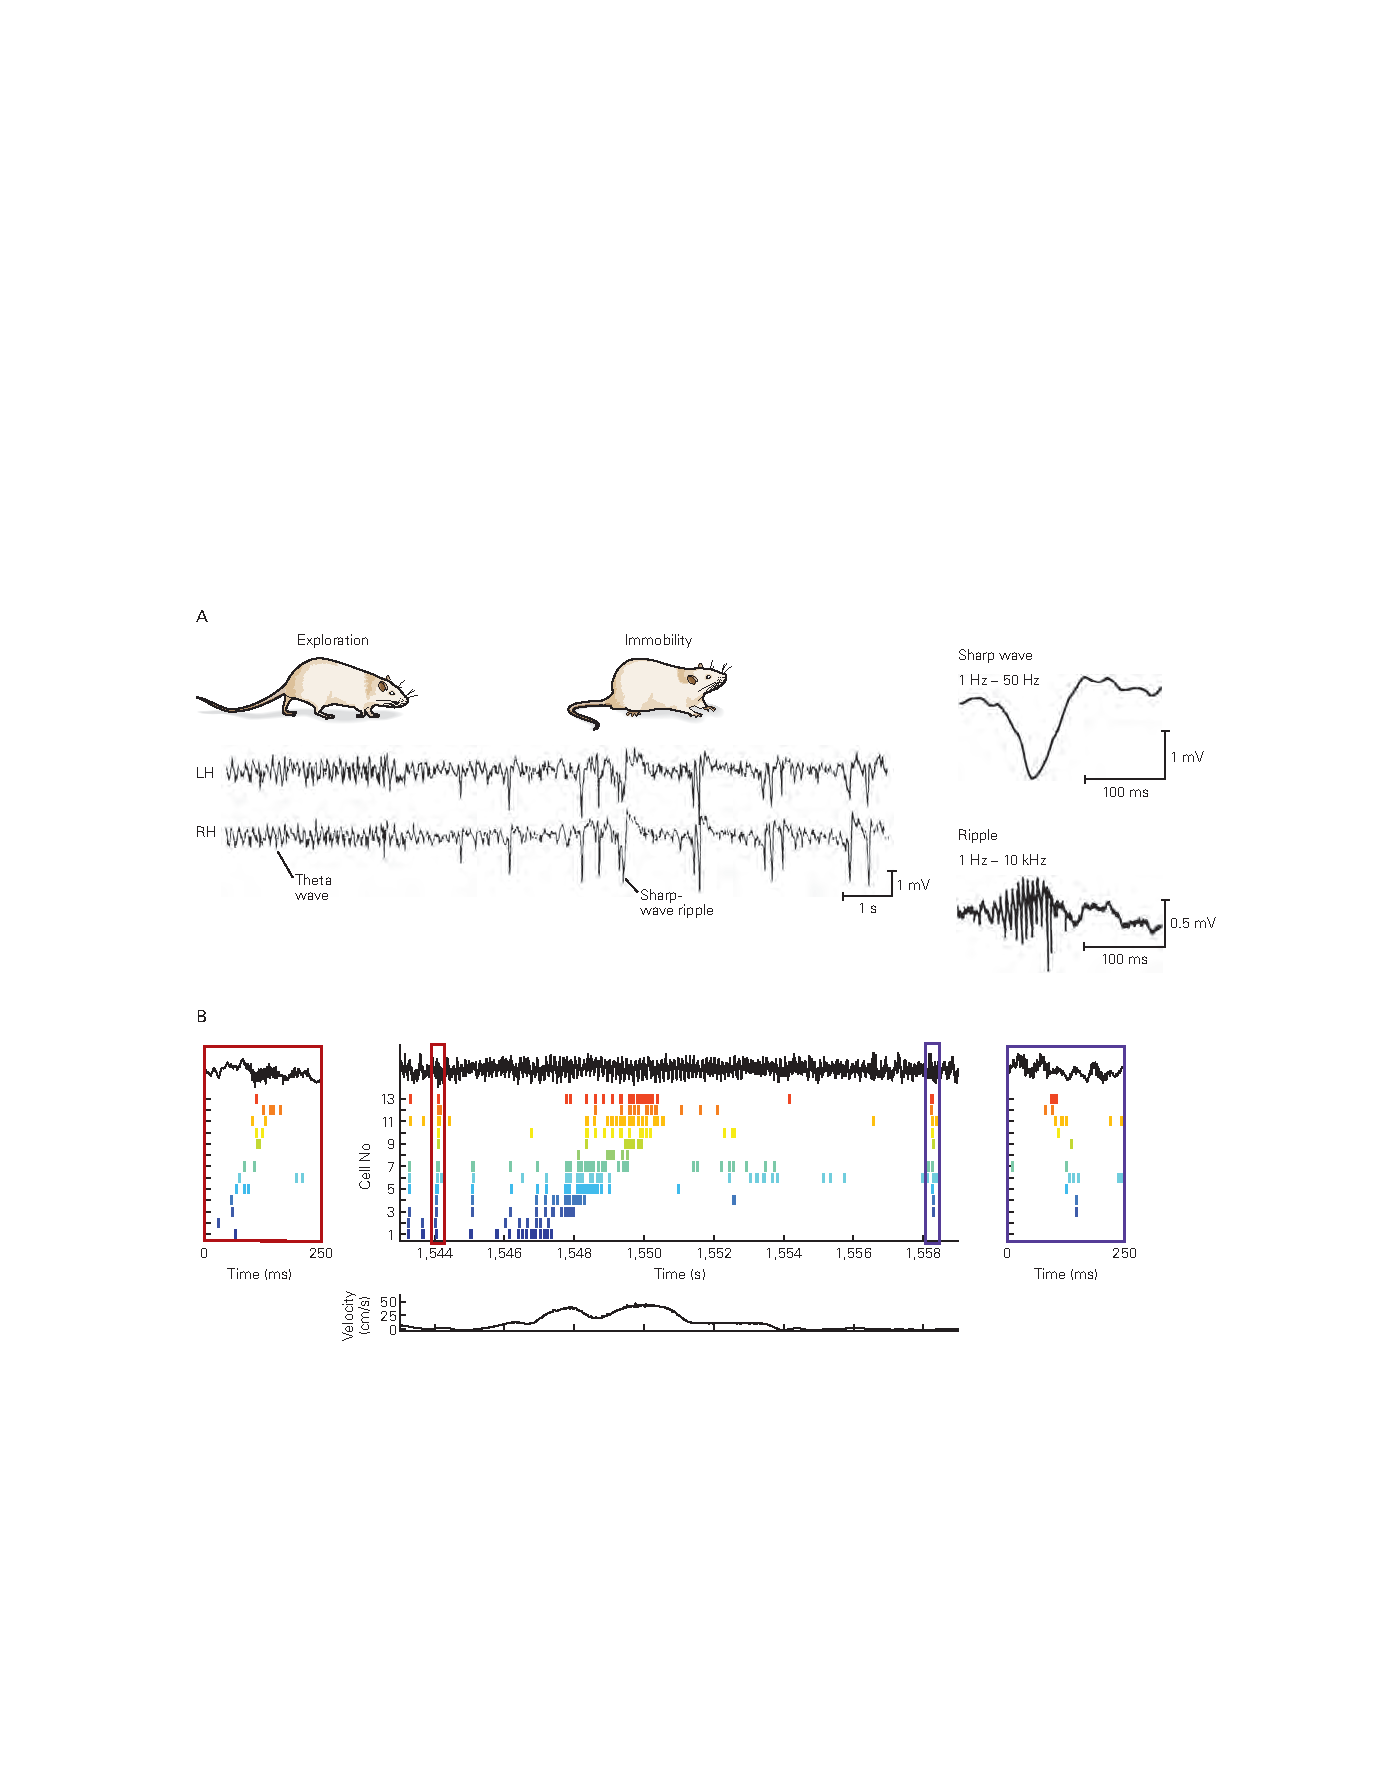
\includegraphics[width=1.0\linewidth]{chap05/fig_5_2}
	\caption{海马\textit{尖波涟漪}和\textit{序列回放}。 
		\textbf{A.} 左图:海马体\textit{局部场电位}活动的行为依赖性(\textit{左海马体}和\textit{右海马体})。
		在探索期间存在$\theta$波,在不动期间存在大的负尖波。 
		右图:从海马\textit{阿蒙角}1 区域记录的尖波和涟漪\cite{buzsaki2015hippocampal,buzsaki1992high}。
		\textbf{B.} 在行为(中图)期间经历的\textit{位置细胞}序列\textit{尖波涟漪}过程中在\textit{前向}(左图)和\textit{反向}(右图)方向上回放。
		老鼠沿着熟悉的轨迹从左向右移动。
		当大鼠在轨迹上时,13 个 \textit{阿蒙角}3 锥体细胞的位置场的脉冲序列显示在单次遍历之前(正向重放;红色框)、期间(中)和之后(反向重放;蓝色框)。
		\textit{阿蒙角}1 局部场电位显示在顶部(黑色痕迹),动物的速度显示在下方\cite{diba2007forward}。}
	\label{fig:5_2}
\end{figure}


值得注意的是,尖波涟漪在最近学习后的休息期间很突出,例如在探索环境之后,锐波涟漪很突出。
对在这些短尖波波纹内(50 毫秒到 500 毫秒)活跃的位置细胞活动的空间解码表明,海马神经元通过最近探索的环境重演或重播离散轨迹。
尽管这些轨迹复制了穿越空间的路径,但重播的活动序列在几个方面与主动探索期间观察到的不同。


首先,锐波波纹内的重放序列被时间压缩,发生速度比探索期间快 10 到 20 倍(图~\ref{fig:5_2}B)。 
其次,它们可以发生在与行为空间轨迹相同的方向(正向重播)或相反的方向(反向重播)。
因此,解码单个探索后的 200 毫秒尖波波纹重播事件可能会揭示一个虚拟的心理轨迹,该轨迹跨越 2 到 4 秒的行为时间,从它的经历中回放。
重放被认为代表了一种心理排练形式,通过这种形式,某些记忆逐渐得到巩固,因此可能是海马体在记忆中的作用的一个重要方面。



\section{神经回路基序为信息处理提供了基本逻辑}

神经元往往与附近的神经元和远端大脑区域的神经元高度互连。
由于许多揭示精细解剖结构的新方法,神经元连接的知识(称为连接组学)正在迅速扩展。
神经元互连的模式有多种。


从一个区域到另一个区域的连接,例如从丘脑到初级视觉皮层,被称为前馈(图~\ref{fig:5_3}A)。 
前向被定义为从更外围或主要区域(例如视网膜、丘脑或初级视觉皮层)延伸到具有更复杂响应特性的更高区域,例如选择性地响应特定目标的视觉区域。
在大多数情况下,具有前馈连接的两个区域也具有反馈连接;
例如,从初级视觉皮层到丘脑有许多连接。
局部连接通常从一个神经元延伸到另一个神经元,最终循环回到原始神经元。
这种循环连接称为循环。
许多神经元都参与了所有这些类型的连接(前馈、反馈和循环),但分别考虑这些不同连接基序的功能含义是有用的。


\begin{figure}[htbp]
	\centering
	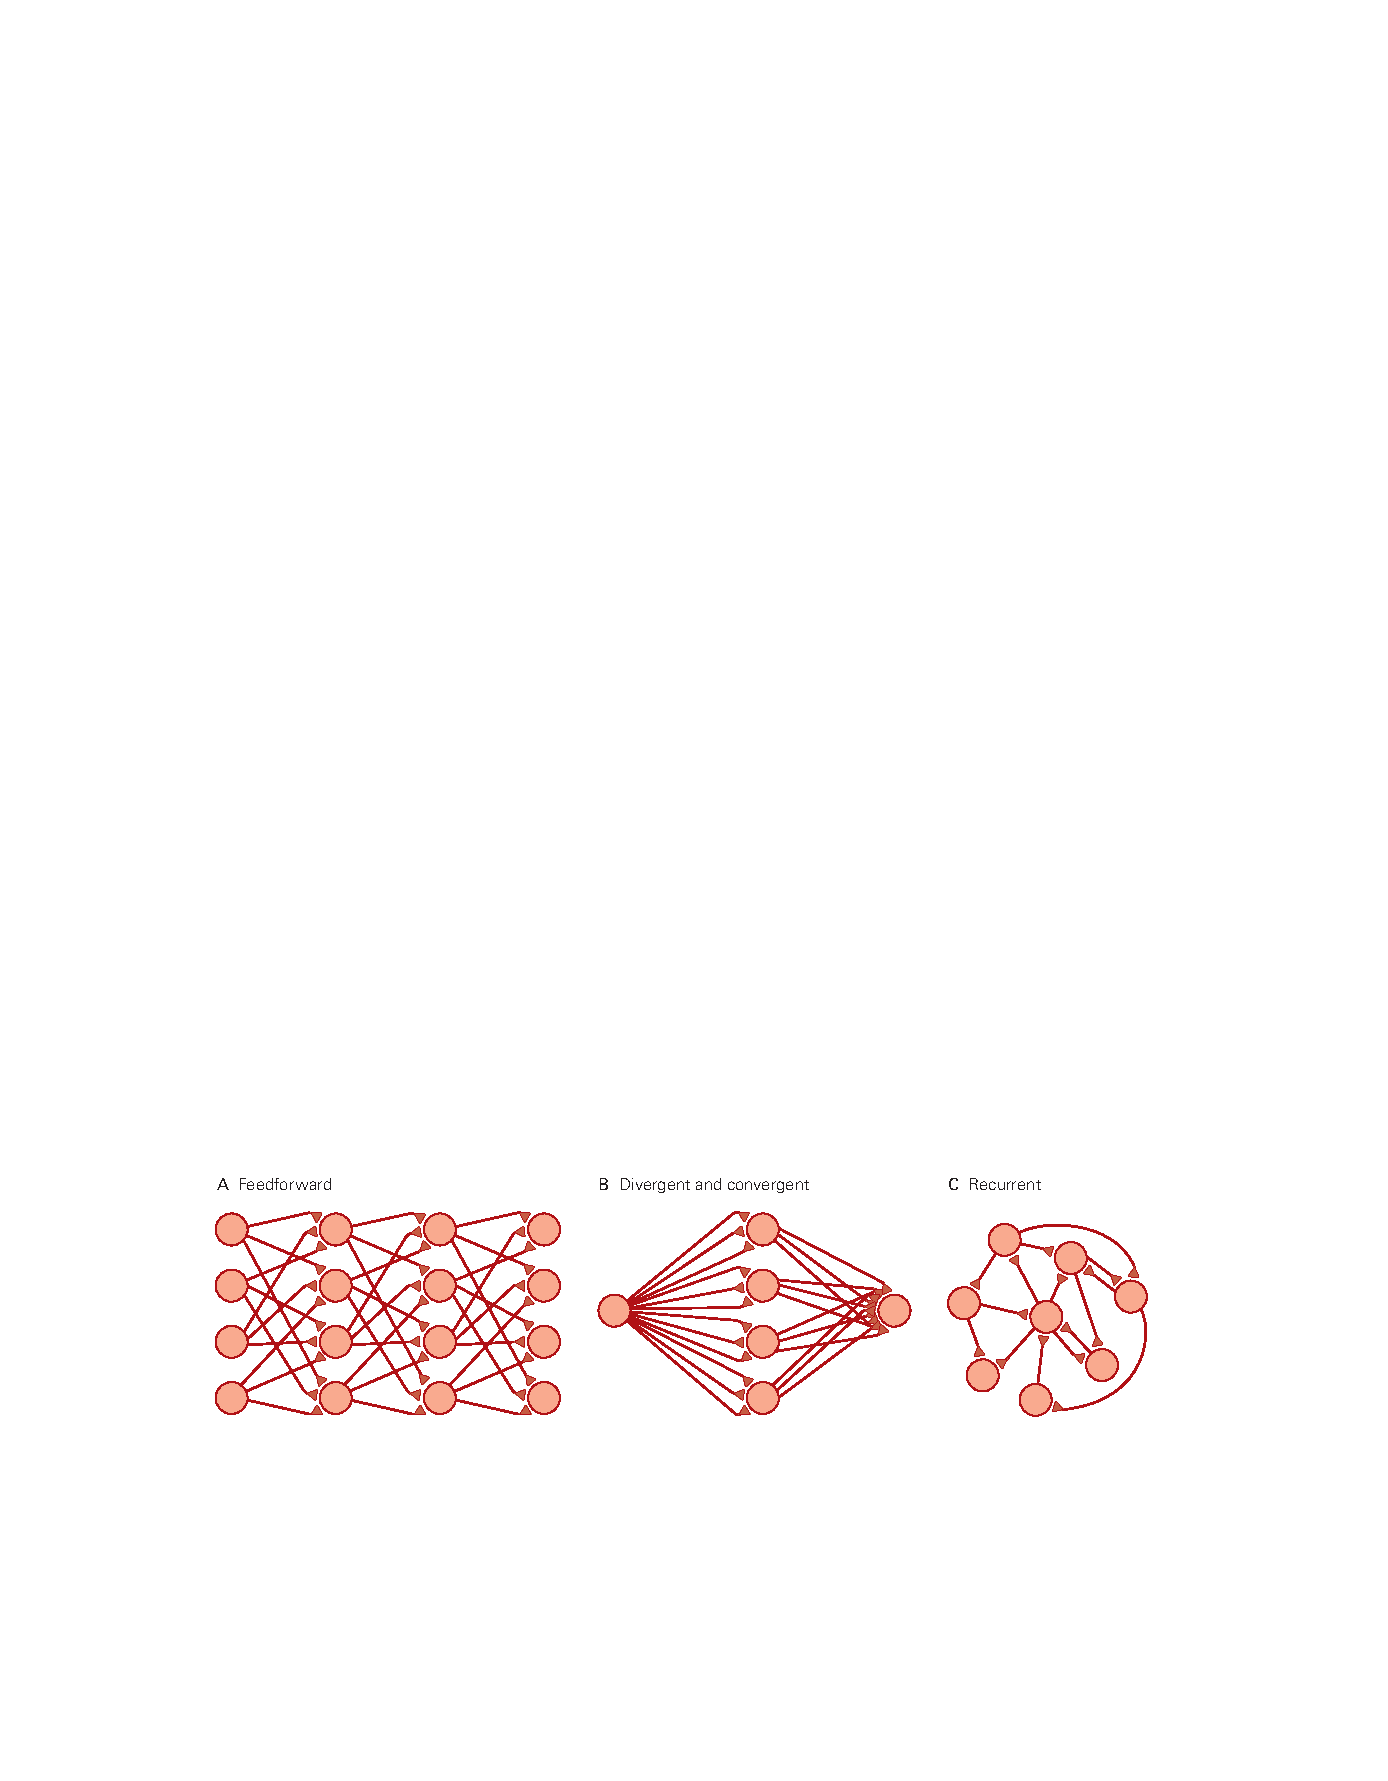
\includegraphics[width=1.0\linewidth]{chap05/fig_5_3}
	\caption{四种基本的神经回路图案。 
		\textbf{A.} 一种\textit{前馈}回路,其中突触连接在一个方向上从神经元的一个处理级别延伸到另一个处理级别。
		\textbf{B.} \textit{发散}的前馈连接描述了少量的突触前神经元连接到大量的神经元。
		\textit{汇聚}连接描述了连接到较小数量的大量突触前神经元。
		\textbf{C.} 在\textit{循环网络}中,神经元之间的多个方向发生突触连接,形成通过回路的循环通路。}
	\label{fig:5_3}
\end{figure}


神经元之间的连接可以是兴奋性的或抑制性的。
通常,兴奋性连接会导致神经放电增加,而抑制性连接会导致神经放电减少。
许多神经回路从成百上千个突触中接收到强烈的兴奋驱动。
如果不通过抑制来检查,这种突触兴奋将导致不稳定的神经活动。
兴奋和抑制的接近平衡是神经回路的一个共同特征,可以增强它们的计算能力。
然而,如果兴奋和抑制之间的平衡没有得到适当维持,这种微调可能会使回路容易产生癫痫发作活动,就像在癫痫期间发生的那样。


在哺乳动物中,视觉信息在一系列通常被近似为具有前馈回路的大脑区域中进行处理。
前馈回路可以以复杂的方式处理信息,例如从复杂的视觉场景中提取和识别目标,但它们不能产生持续的、动态的活动模式。
为此,需要循环回路(图~\ref{fig:5_3}C)。


在前馈回路中,可以识别两个子主题:发散连接和收敛连接(图~\ref{fig:5_3}B)。 
在发散连接中,接收给定类型输入的神经元数量超过提供该输入的神经元数量,因此在突触前输入神经元中编码的信息在突触后输出神经元中扩展。
在会聚连接中,许多突触前神经元将输入发送到数量较少的突触后神经元。
发散和收敛连接的最突出例子是由小脑提供的,如后所述。



\subsection{视觉处理和目标识别取决于前馈表示的层次结构}

视觉信息在大量分层排列的大脑区域中进行处理(图~\ref{fig:5_4})。
从视网膜产生的主要感觉输入向上移动,神经元对越来越复杂的视觉特征组合做出反应,最终导致对复杂物体(例如面部)的选择性。
大量研究致力于确定视觉层次结构所基于的原则。
机器视觉中人工神经网络模型的发展已被证明是解决该问题的有益类比。


\begin{figure}[htbp]
	\centering
	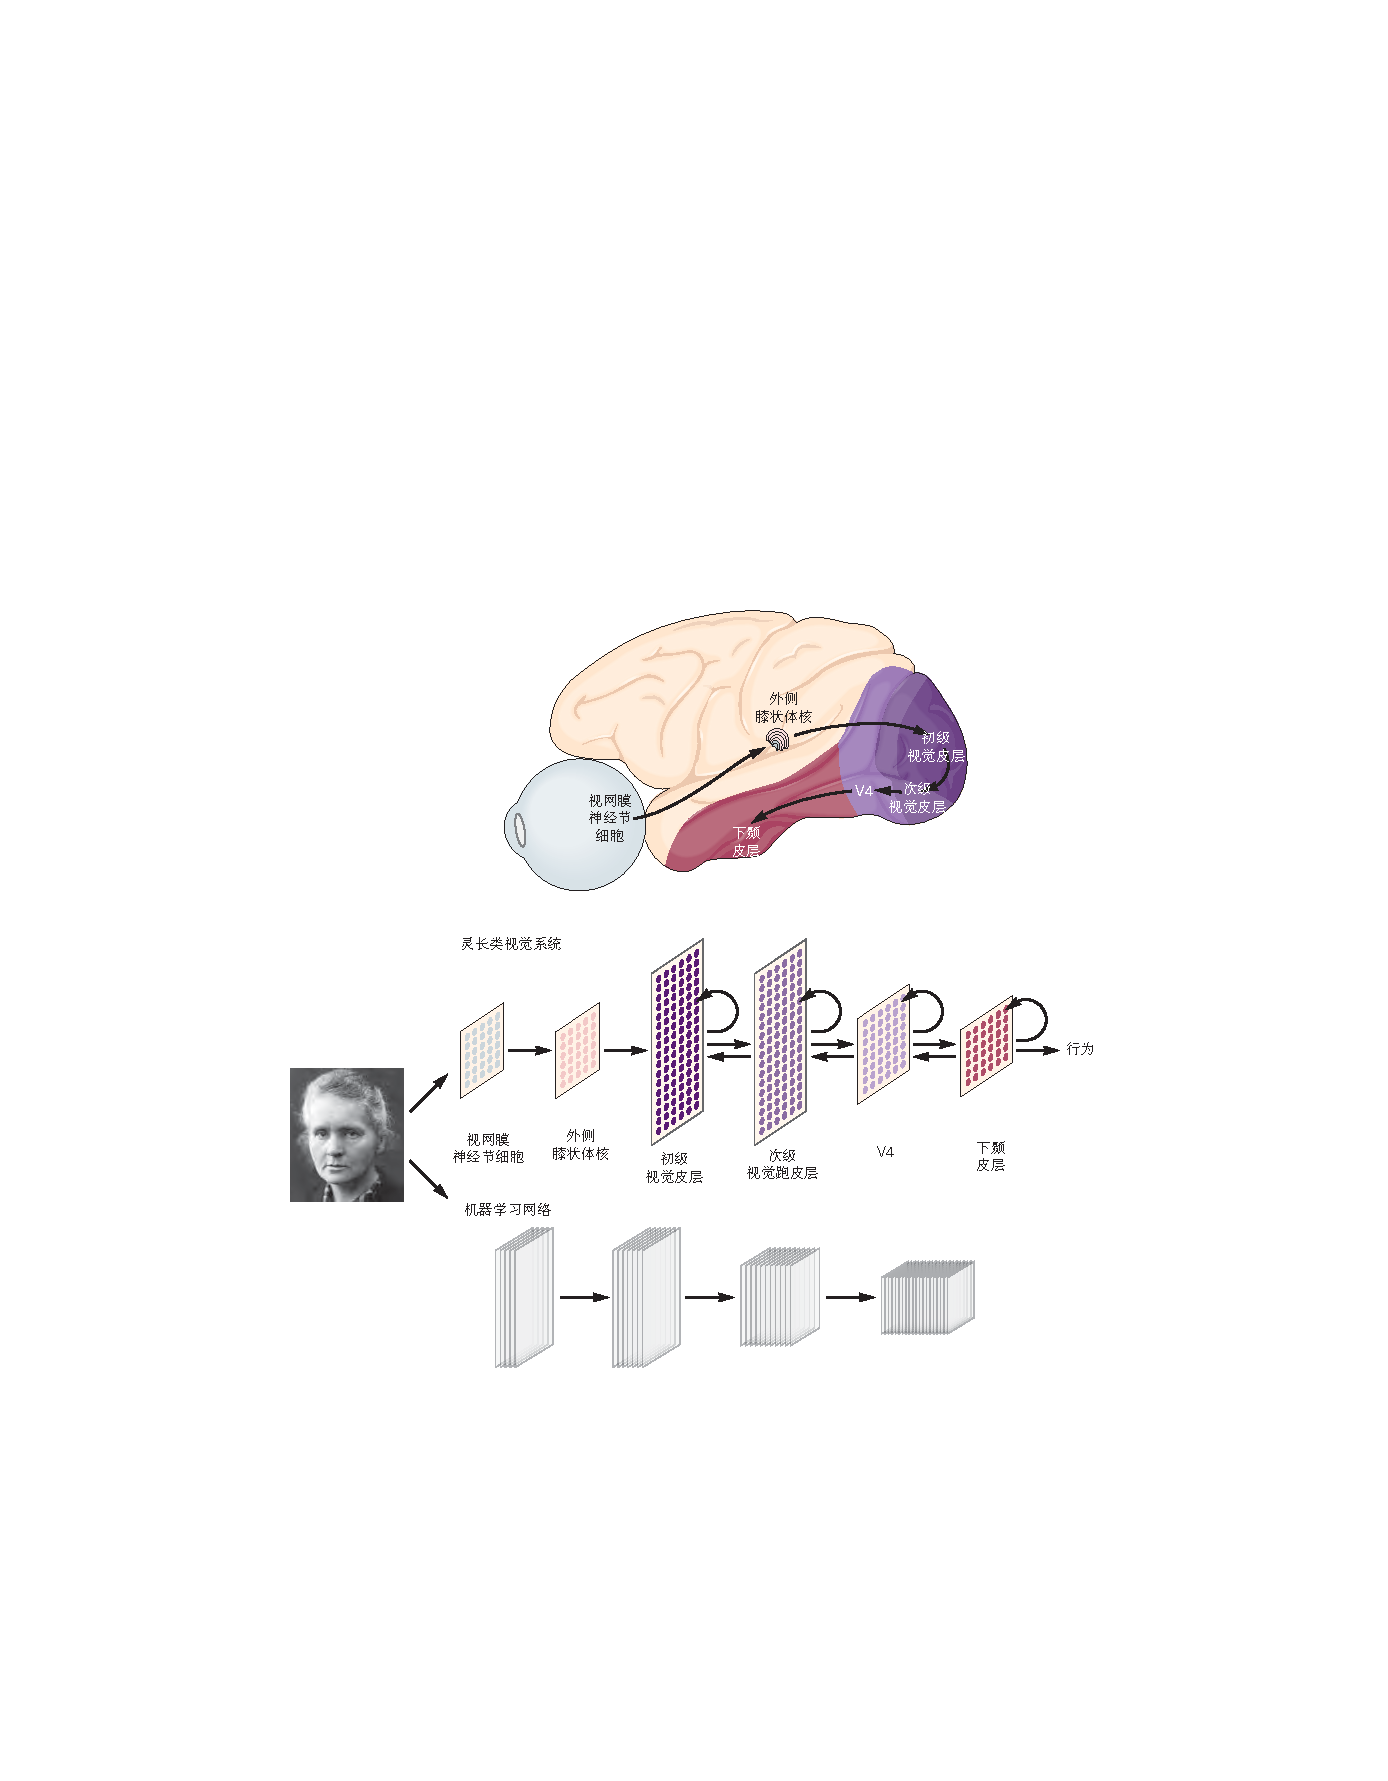
\includegraphics[width=1.0\linewidth]{chap05/fig_5_4}
	\caption{生物和机器学习网络的比较。
		在视觉系统中,多个大脑区域形成一个层次结构,其中串联的神经元对更复杂的目标逐渐具有选择性。
		灵长类视觉系统通路中的区域代表\textit{视网膜神经节细胞}、丘脑的\textit{外侧膝状体核}、腹侧流视觉区域(\textit{初级视觉皮层}、\textit{次级视觉皮层} 和 V4)和\textit{下颞皮层}。
		每个区域的神经元\textit{数量}各不相同(由彩色圆点表示),但它们的\textit{选择性}稳步增加。
		机器学习网络通路表示经过训练以识别图像中目标的前馈网络层。
		越来越多的堆叠子层表明机器学习网络不同区域的选择性增加,反映了对更丰富的视觉特征阵列的选择性。
		在不同视觉区域记录的响应选择性的层次结构类似于在机器学习网络的相应层中看到的活动\cite{schrimpf2018brain}。}
	\label{fig:5_4}
\end{figure}



从视网膜到丘脑,再到初级视觉皮层,再到与认知相关的最高视觉区域下颞皮层中,视觉神经元选择性地响应视野区域中特定的亮、暗和颜色模式,称为它们的\textit{感受野}。
从视觉处理的最低阶段到最高阶段,神经元的感受野越来越大,选择性也越来越高。
在每个阶段,具有特定类型选择性的神经元往往具有平铺视觉场景的感受野,为所选特征提供全面覆盖。
此外,每个视觉大脑区域中感受野的排列在地形上与视网膜上外部世界图像的布局相匹配,即皮层形成了视野图。


随着感受野的扩大和选择性的提高,神经响应对所选目标或图案精确位置的依赖程度越来越低,而更多地取决于其整体特征。
一般来说,处于视觉处理较高阶段的神经元对视野的较大部分更有选择性地做出反应,并且较少依赖于位置、大小和方向等特征。
这与我们在场景中独立于位置、大小和方向识别目标的能力相关。
例如,在层次结构的最高阶段,神经元可以选择性地响应位于整个视野中的特定面孔,而与面孔的大小或其角度姿势(即头部方向)无关。


平铺、增加感受野大小、增加选择性和减少对视图相关因素的依赖的想法是人工机器视觉网络构建的核心。
这样的网络在某些物体识别任务上可以达到人类水平的性能。
此外,机器在困难图像上所犯的错误模式在某种程度上与人类受试者所犯的错误相匹配。
非人类灵长类动物也可以在与人类相当的水平上执行这些任务,而且有趣的是,沿着目标识别通路的不同视觉区域的记录对应于在视觉处理的相似阶段在人工网络中看到的活动(图~\ref{fig:5_4})。



\subsection{小脑中不同的神经元表征为学习提供了基础}

我们大脑中最丰富的一类神经元是位于小脑输入阶段的大约 500 亿个颗粒细胞,占大脑所有神经元的一半以上。 
小脑是一种对运动协调至关重要的后脑结构,但也涉及自主神经、感觉和认知功能的适应性调节(图~\ref{fig:5_5})。
小脑回路功能障碍可能导致各种神经系统疾病,包括孤独症。
与大多数大脑神经元接收的数千个输入相比,每个颗粒细胞仅接收少量输入(平均四个)。


\begin{figure}[htbp]
	\centering
	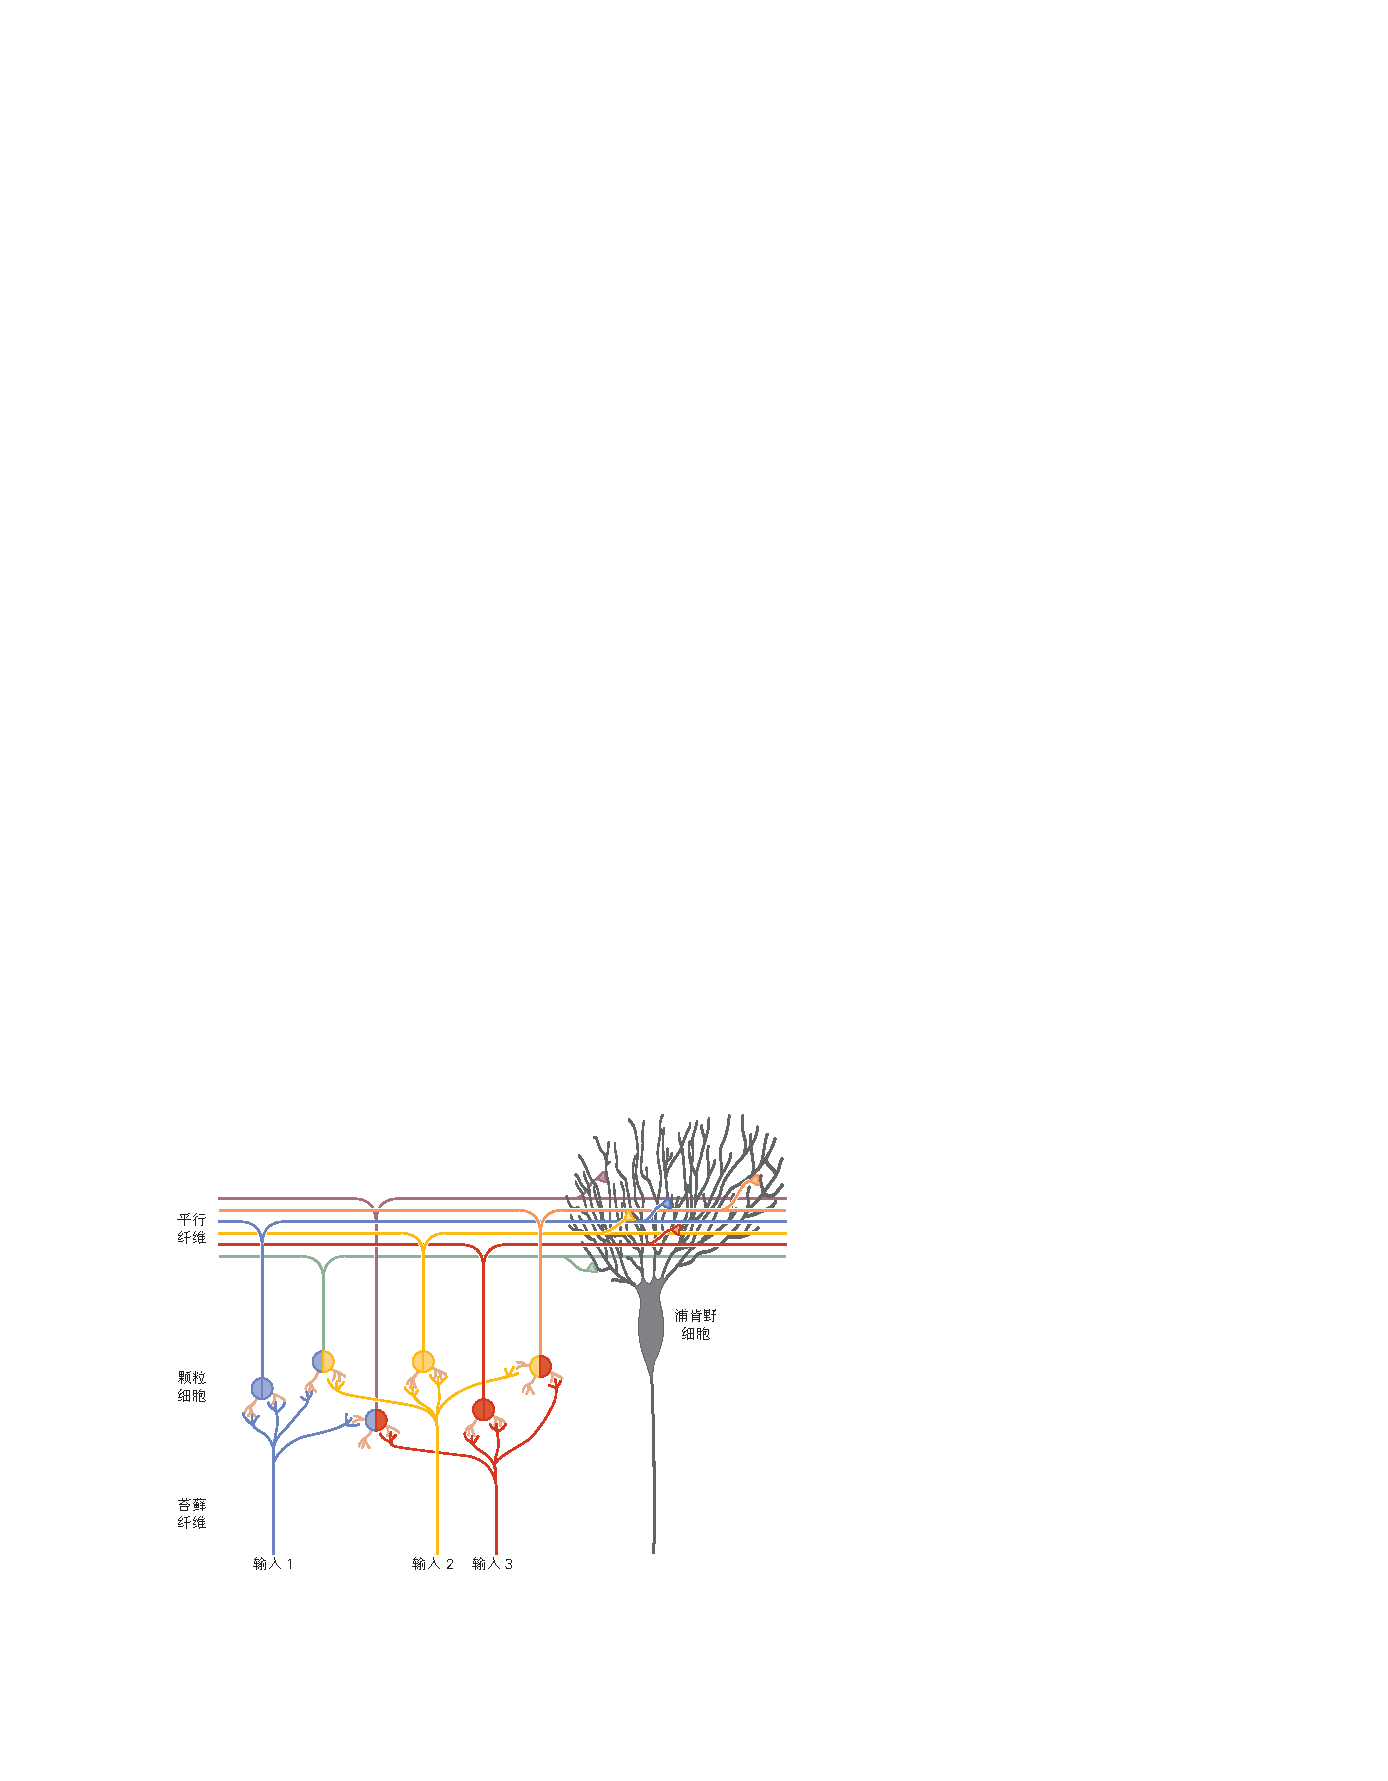
\includegraphics[width=0.9\linewidth]{chap05/fig_5_5}
	\caption{小脑接收来自大脑和脊髓许多区域的输入。
		这些输入统称为\textit{苔藓纤维},在大量\textit{颗粒细胞}中重新编码,这是发散连接的一个例子,允许输入信号的许多可能混合。
		\textit{浦肯野细胞}的树突从轴突(称为平行纤维)中继的数十万个颗粒细胞接收会聚输入。
		浦肯野细胞突触的平行纤维是可改变的,这被认为是运动和可能其他形式学习的重要机制。}
	\label{fig:5_5}
\end{figure}


最近使用神经解剖学追踪和电生理学记录的实验结果表明,汇聚到单个颗粒细胞上的输入通常来自不同的大脑区域。
因此,单个颗粒细胞的放电可能代表大量刺激或事件组合中的任何一种。
例如,细胞可能仅在特定视觉刺激(例如移动的网球)与特定身体部位的运动(例如手腕的弯曲)结合时才会放电。
以这种方式组合不同类型信息的表示称为混合表示。


小脑颗粒细胞提供了\textit{发散前馈连接}的一个极端例子,大约 2 亿个输入纤维(称为\textit{苔藓纤维})携带的信息混合并扩展到 500 亿个\textit{颗粒细胞}上。
需要如此大的表示来处理可以组合多个信息通道的许多不同方式。
例如,表示 100 个不同输入通道中的 2 个的所有可能组合需要 100 × 99/2,即 4,950 种不同的响应类型。
需要所有三元组的表示将这个数字推高到 15 万以上,并且对于四个或更多的组合,这个数字会迅速增加。
因为大量可能的组合很难从基因上指定,所以通常认为苔藓纤维与其颗粒细胞目标的分配在很大程度上是随机的。


该分析表明,小脑颗粒细胞的作用是以多种可能的方式\textit{组合}大量输入通道。
这种表示显然有助于根据刺激和动作组合的共现进行推理和生成动作。
然而,要发挥作用,必须以某种方式从大量颗粒细胞中读出这些信息。


小脑细胞的\textit{读出}是由浦肯野细胞完成的,浦肯野细胞是小脑皮层的输出神经元。
与颗粒细胞输入端高度不同的连接相反,颗粒细胞和浦肯野细胞之间的连接提供了一个极端的\textit{汇聚}例子。
单个浦肯野细胞接收来自超过十万个颗粒细胞的输入。
\textit{大卫$\cdot$马尔}和\textit{詹姆斯$\cdot$阿尔布斯}在 1970 年代提出的小脑功能理论认为,这种融合使\textit{浦肯野细胞}能够从颗粒细胞提供的极其丰富的表征中提取有用的信息。
通过这样做,例如,浦肯野细胞可能成为人类惊人的能力的基础,可以形成运动技能所需的许多复杂关联,例如骑自行车或演奏乐器。
然而,为了在各种条件下提取对多种目的有用的信息,浦肯野细胞提供的读数必须具有适应性。
如后面部分所述,这种适应性是由颗粒细胞和浦肯野细胞突触之间的\textit{突触可塑性}提供的。



\subsection{循环回路是持续活动和整合的基础}

神经元天生健忘。 
瞬态突触输入通常会引起短暂的响应,这种响应会在几十毫秒内衰减。
这种衰变的时间过程由神经元的一种内在特性决定,称为\textit{膜时间常数}(第~\ref{chap:chap9}~章)。
那么神经活动模式如何持续足够长的时间以支持认知操作,例如在几秒钟、几分钟甚至更长时间内完成记忆或决策制定?


例如,考虑在挤满大声说话的拥挤房间中尝试检测您是否听到熟悉的声音。
当您聆听时,您可能偶尔会发现一些类似于您正在寻找的声音,但这本身并不能确定。
然而,随着时间的推移,您可能会积累足够的证据来得出结论。
这个证据积累过程需要整合,这意味着必须维护一个运行总和,并在检测到额外证据时增加。
整合需要计算(加法)和记忆来计算和维护运行总和(第~\ref{chap:chap56} 章)。


对于执行整合的神经回路,瞬态输入必须产生即使在输入消失后也能维持在恒定水平的活动。
这种持续的活动提供了对瞬态输入的记忆。
如前一段所述,整合回路可用于积累信息,但它们也需要用于非认知任务,例如保持固定身体姿势所需的恒定肌肉张力。
研究得最好的神经整合器之一是允许人类和动物保持眼睛恒定注视方向的回路,即使在黑暗中也是如此。
事实上,可以研究从鱼类到灵长类动物广泛物种的眼球运动,这极大地促进了进步。
此外,动眼神经系统的相对简单性促进了实验研究和理论研究之间富有成果的对话(动眼神经系统在第~\ref{chap:chap35} 章有更详细的描述)。


动眼神经系统中整合回路的存在最初是由来自神经元记录的令人费解的观察结果提出的(图~\ref{fig:5_6}A)。
控制眼部肌肉的动眼神经元会瞬时增加动作电位放电以引起眼睛的运动,但也会表现出将眼睛保持在固定位置所需的持续动作电位放电。
例如,投射到使眼睛向左移动的眼部肌肉的运动神经元将在注视保持在中心左侧时以高速率放电,而在注视保持在中心右侧时以低速率放电。
令人困惑的是,投射到动眼神经元的上丘和脑干中的运动前神经元仅在眼球运动之前短暂放电。
它们不显示任何与眼睛位置相关的持续活动。
那么这种持续的活动是如何产生的呢?


\begin{figure}[htbp]
	\centering
	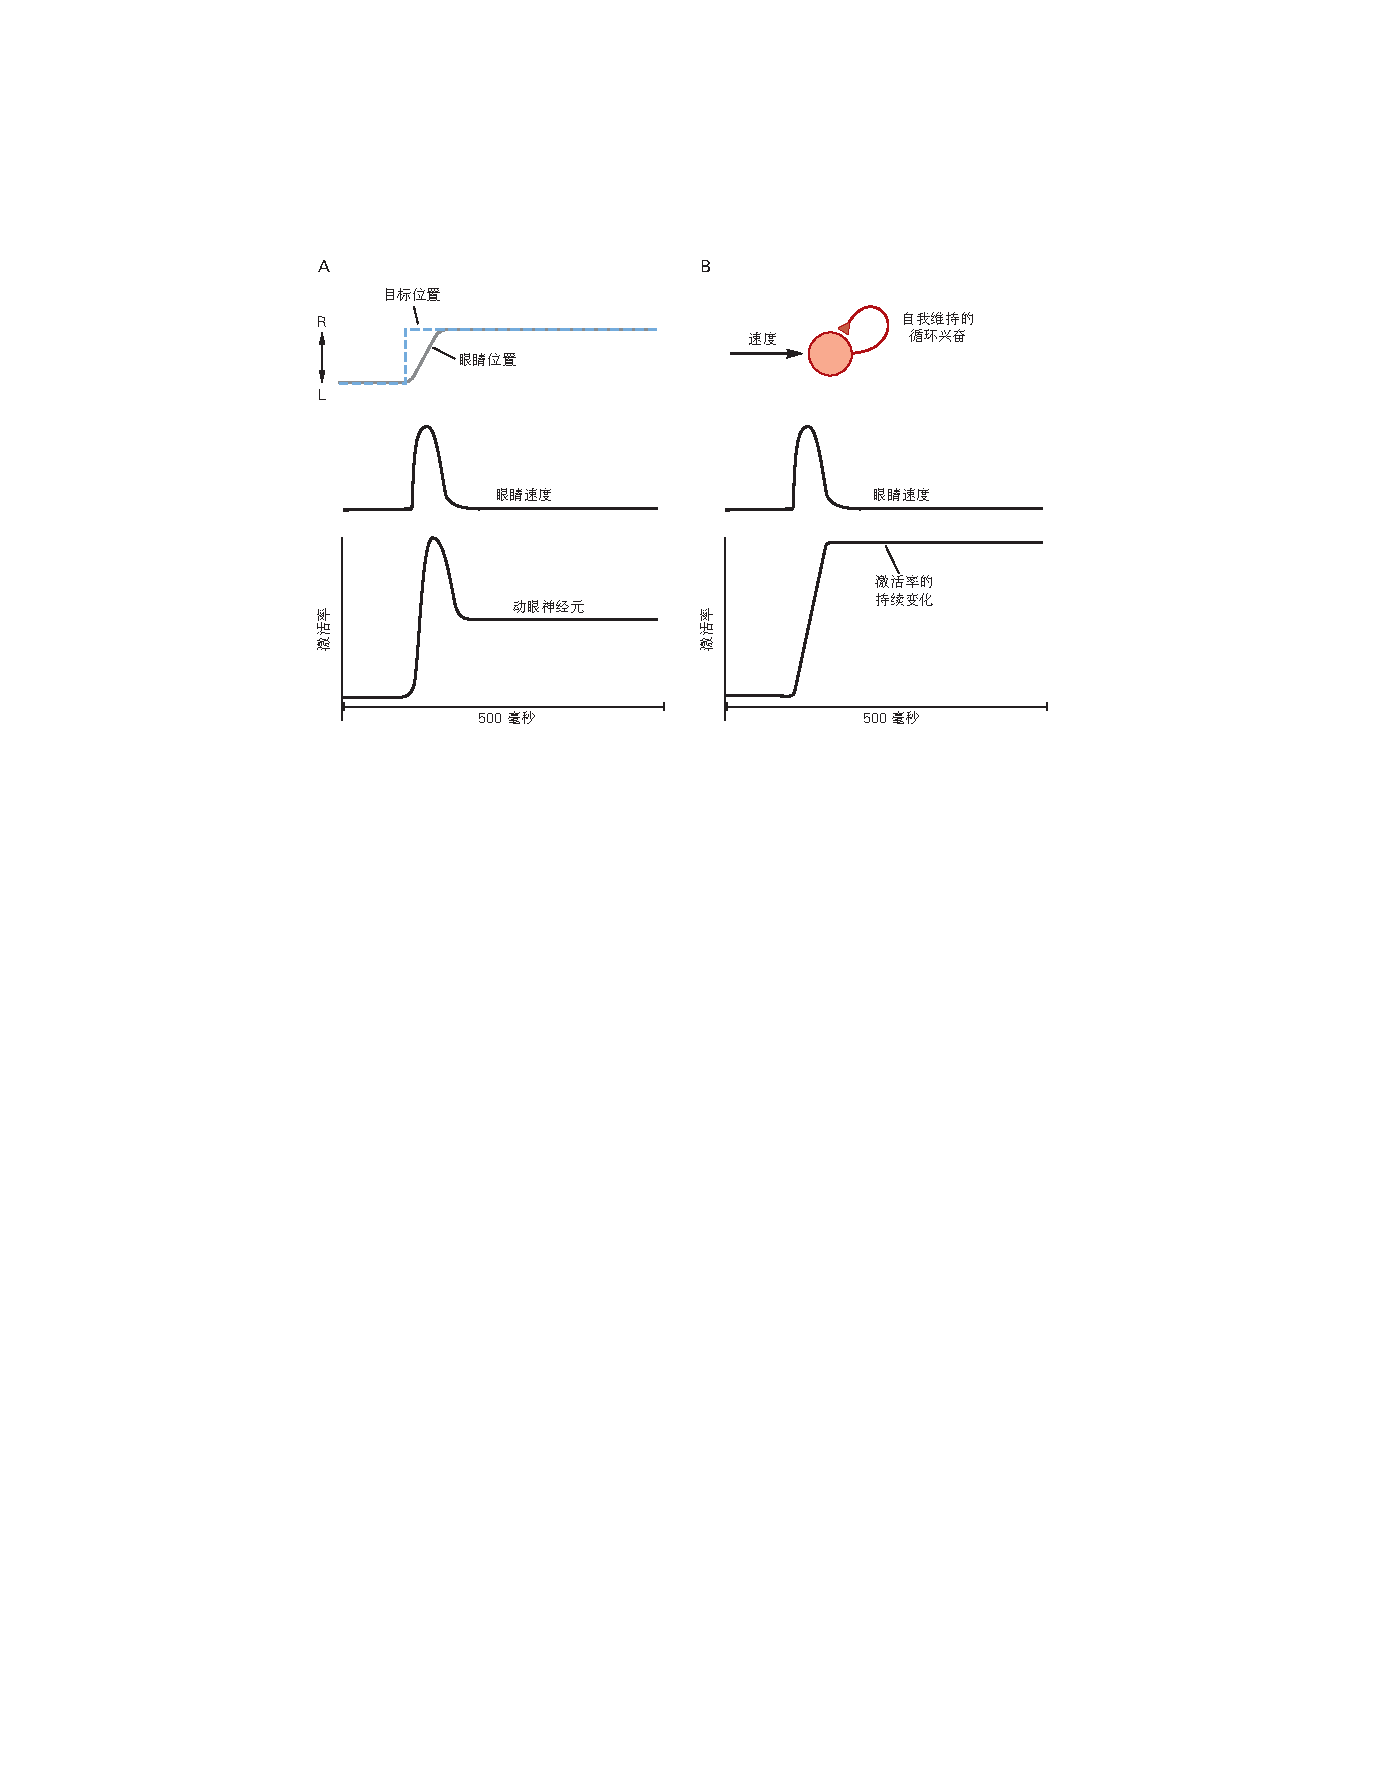
\includegraphics[width=0.9\linewidth]{chap05/fig_5_6}
	\caption{维持眼睛位置需要循环回路和持续的神经活动。
		\textbf{A.} 上图:\textit{扫视}眼球运动包括眼球速度的快速运动变化,以将目标带回凝视中心。
		随后持续改变眼睛位置以将中央凹保持在目标上。
		蓝色虚线表示\textit{目标位置},灰色线表示眼球运动和随后在新位置对目标的注视。
		下图:动眼神经元表现出与眼睛速度相关的短暂活动以及与眼睛位置相关的持续活动。
		\textbf{B.} 反复激发可以解释输入的短暂脉冲(例如眼速信号)如何通过类似于数学积分的过程导致放电率的持续变化。}
	\label{fig:5_6}
\end{figure}


一个现在得到了强有力支持的早期猜想,是稳定的眼睛位置信号是由整合瞬态眼球速度信号的脑干神经元计算的。 
这些神经元接收速度信息并向维持眼睛位置的动眼神经元提供稳定的输出。 
猴子某些脑干核团(包括内侧前庭核和舌下舌前核)的损伤或失活导致眼球运动后无法保持稳定的水平眼位,表明神经整合回路位于这些结构内。 
人类这些脑干结构的损伤会导致同样的问题,临床上称为凝视诱发性眼球震颤(第~\ref{chap:chap35}~章)。


神经回路如何进行整合?
一种可能性是整合得到专门内在神经元特性的支持,这些特性有效地延长了神经元\textit{膜时间常数},允许短暂的输入产生持续的输出。
已经描述了涉及不同电压激活离子通道的多种候选机制。 
然而,使用允许直接控制记录神经元的膜电压的细胞内记录的研究表明,即使神经元的电压激活通道被阻断,持续的位置相关信号也会持续存在。 
第二种可能性是整合源于突触耦合神经元网络之间的相互作用。 
金鱼的细胞内记录通过显示突触输入水平随眼睛位置而变化来支持这一观点。


什么类型的神经网络能够执行整合的问题已经在理论研究中得到广泛探索。 
已考虑的一类模型依赖于循环连接,特别是一群相互激发的神经元。 
这种类型的弱耦合网络响应输入脉冲,其活动迅速衰减。 
增加反复激发的强度会增加一些原本会衰减的活动,从而延长群体反应的持续时间。
如果循环激励增加到由瞬态输入建立的循环激励精确抵消衰减的程度,则响应可以无限期地持续。 这需要微调网络参数。


在一个完美调谐的网络中,一个瞬态输入脉冲会导致激活率发生变化,这种变化在没有进一步输入的情况下会永远持续下去。 
等效地,这样的群体计算它接收到的输入的运行整合(图~\ref{fig:5_6}B)。
如果网络中的瞬态激励没有得到完美调整,而是稍微变弱,则输入会产生缓慢衰减的放电率变化。 
在黑暗中,眼睛位置往往会在大约 20 秒内漂移回中心,这表明神经整合器没有完美调整,但它调整得足够好,可以将典型神经元的大约 20 毫秒时间常数延长一个 约 1 千的系数。


循环网络模型再现了在生物整合器回路中观察到的一些核心特性这一事实已经启动了更详细和更现实的网络模型的开发,并通过实验测试了此类模型的预测。
这些努力还突出了在神经回路的结构和功能之间建立详细联系所涉及的挑战。
即使在使用各种系统和方法进行了数十年的深入研究之后,关键问题仍然存在。


例如,动眼神经整合器回路通常包含两类相反的神经元,随着眼睛位置在给定方向上的变化,一类神经元的放电率增加,另一类神经元的放电率降低。 
这种排列不仅限于动眼神经整合器,还存在于与决策制定和工作记忆有关的皮层区域。
模型表明,这些对立群体之间的相互抑制可以在维持活动和融合方面发挥作用。 
尽管解剖学研究为这一观点提供了一些支持,但对金鱼的研究表明,即使对立群体之间的联系被移除,整合仍然完好无损。


另一个关键问题涉及调整积分器网络的机制。
实验研究表明,整合器网络会根据经验进行修改;
换句话说,它们是可调的。 
尽管这种调整可能是通过神经元之间突触连接强度的变化而发生的,但尚未获得直接证据。 
简而言之,尽管已经了解了很多关于如何实现集成的知识,但在任何特定实例中实际支持集成的网络架构的细节仍有待确定。


详细了解我们如何保持眼睛的位置本身就是一个重要的目的,具有临床意义。 
然而,如前所述,此处找到的解决方案可能同样适用于认知功能,包括短期记忆和决策制定。
大量神经元的光学成像以及对其活动的时间精确操作和详细的解剖学重建,再加上网络功能的理论模型,可能很快就会提供答案。



\section{学习和记忆取决于突触可塑性}

经验可以修改神经回路以支持记忆和学习(第~\ref{chap:chap3}~章)。
人们普遍认为,负责学习和记忆的经验依赖性变化主要发生在突触上。
已经确定了多种形式的突触可塑性,其中每一种都可能支持一组不同的功能。


正如可塑性有多种形式一样,学习也有多种形式。
可以根据所提供信息的数量和类型来定义不同的学习形式。
在监督学习中,会给出有关执行任务所需行为的明确指示。
另一方面,在强化学习中,仅提供正奖励或负惩罚来指示该任务是否正确执行。
最后,无监督学习根本不涉及任何指导性信息,而是在没有监督的情况下根据其内在结构组织输入数据。
在以下部分中,我们将讨论涉及赫布可塑性的无监督学习示例和小脑强化学习示例(学习和记忆的各种类型及其细胞和回路机制在第~\ref{chap:chap52}~至~\ref{chap:chap54}~章中有详细描述)。



\subsection{突触输入的主导模式可以通过赫布可塑性来识别}

皮层神经元接收来自数千个其他神经元的突触输入,并将这些信息组合成动作电位模式。
每个突触的突触传输强度决定了来自许多输入的信息如何组合以影响神经元的放电。
将所有突触的强度设置为零显然会产生一个无功能用途的无信息神经元。
同样,将它们设置为非零值以提取由随机噪声主导的信号也不会产生有价值的信号。
相反,神经元可以通过提取其输入携带的信息中最有趣的方面来最好地发挥有用的功能。
对一种称为\textit{赫布可塑性}形式的理论分析表明,这可能以一种无监督的方式发生。


1949 年,\textit{唐纳德$\cdot$赫布}提出,当给定的神经元突触前输入与足够数量的协同输入合作,导致该神经元激发动作电位时,突触应该增强。
赫布突触可塑性的证据已从许多研究中获得(第~\ref{chap:chap54}~章)。 
就其本身而言,赫布可塑性会使突触越来越强,因此必须存在某种其他形式的可塑性来防止这种情况发生。 
这种可塑性的补偿形式被称为稳态,实验也揭示了这些形式的可塑性。 
理论分析表明,\textit{赫布可塑性}和\textit{稳态可塑性}的组合可以调整突触,无需任何额外的监督信号,因此它们提取相对于其他组合调制程度最高的神经元输入组合(图~\ref{fig:5_7})。 
这是这些输入携带的最有趣信号的合理候选者,因此,赫布可塑性为神经元提供了一种确定和提取此类信号的方法。


\begin{figure}[htbp]
	\centering
	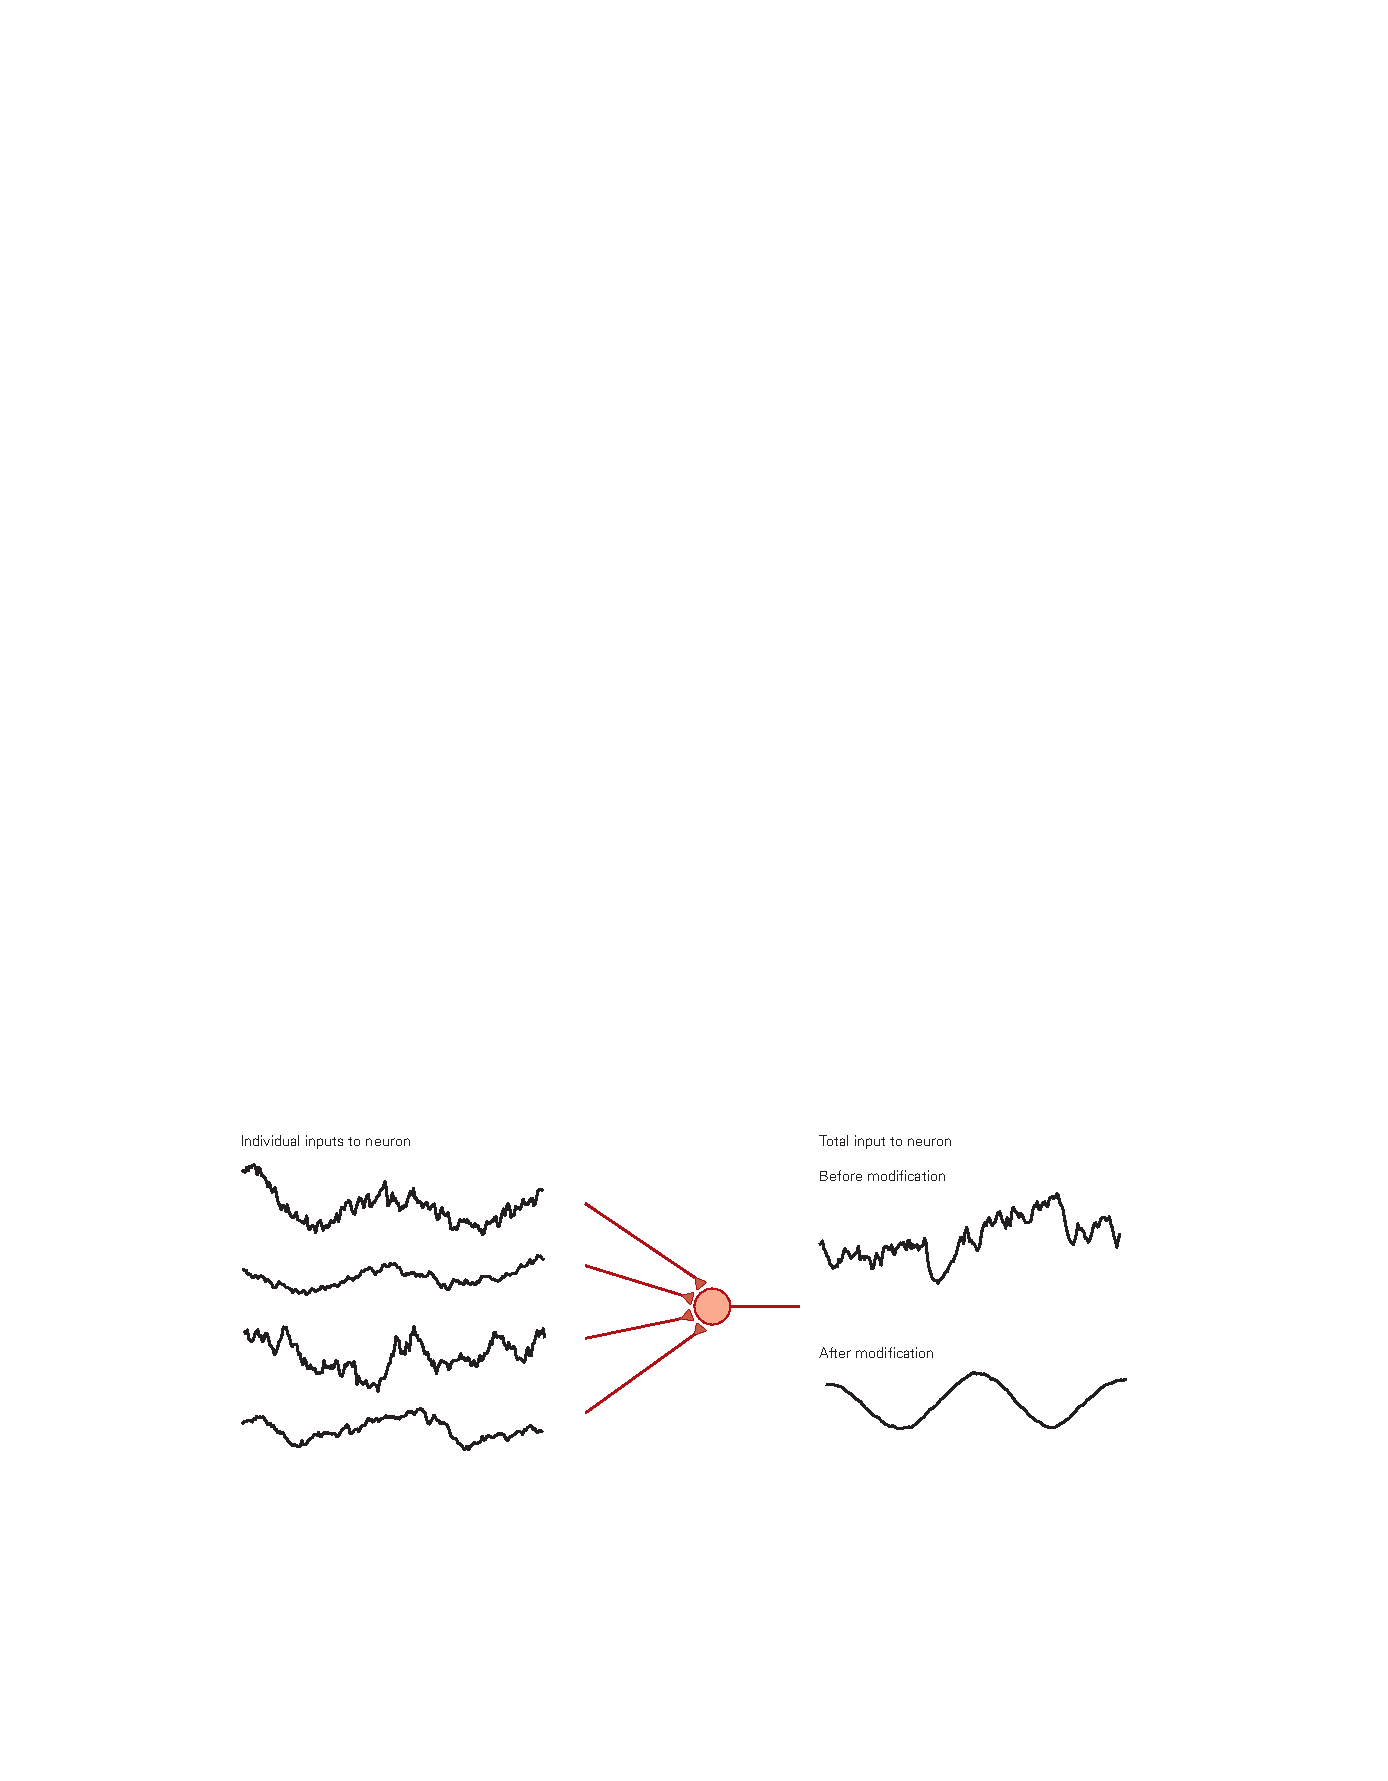
\includegraphics[width=1.0\linewidth]{chap05/fig_5_7}
	\caption{赫布可塑性可以识别神经元的相关输入信号。
		在这个例子中,一个神经元接收 100 个输入;
		显示了其中四个的激活率(左)。
		每个输入速率都有噪声,但在噪声中包含正弦信号。
		输入速率乘以突触强度(棕色三角形),然后求和以产生神经元的总输入(右)。
		在\textit{赫布可塑性}发生之前,突触具有随机权重,导致噪声轨迹;
		修改后,总输入揭示了潜在的正弦信号。}
	\label{fig:5_7}
\end{figure}


\subsection{小脑的突触可塑性在运动学习中起着关键作用}

尽管缺乏对小脑如何促进复杂人类运动技能的详细了解,但人们对其在简单形式的运动学习中的作用了解很多。
其中研究最透彻的是一种被称为\textit{延迟性眨眼条件反射}的范例,其中中性感官刺激(例如光或音调)与厌恶的\textit{非条件刺激}(例如向眼睛吹气)反复配对。
经过几天的此类训练,动物学会闭上眼睛以响应先前的中性刺激(光线或音调),称为\textit{条件刺激},以期待\textit{非条件刺激}(吹气)。
眼睑闭合的时间对于\textit{条件刺激}发作和\textit{非条件刺激}之间的延迟具有高度特异性。


眼睑条件反射一直是理解小脑功能的一个非常有用的范例,因为它以一种特别清晰的方式映射到小脑回路的结构上(图~\ref{fig:5_8})。
有关\textit{条件刺激}的信息首先由小脑颗粒细胞编码,然后传递给浦肯野细胞。
\textit{非条件刺激}由一个完全独立的输入通路编码,称为橄榄小脑或攀爬纤维系统。
与来自颗粒细胞的数千个输入相反,每个浦肯野细胞从称为下橄榄的脑干核接收单个强大的攀爬纤维输入。
电生理记录显示,向小脑某一特定区域输入的攀爬纤维表示\textit{非条件刺激}的发生,即刺激角膜的刺激。
这一发现之所以成为可能,是因为攀爬纤维在浦肯野细胞中引起了一种独特的超阈值反应,称为复杂尖峰。


\begin{figure}[htbp]
	\centering
	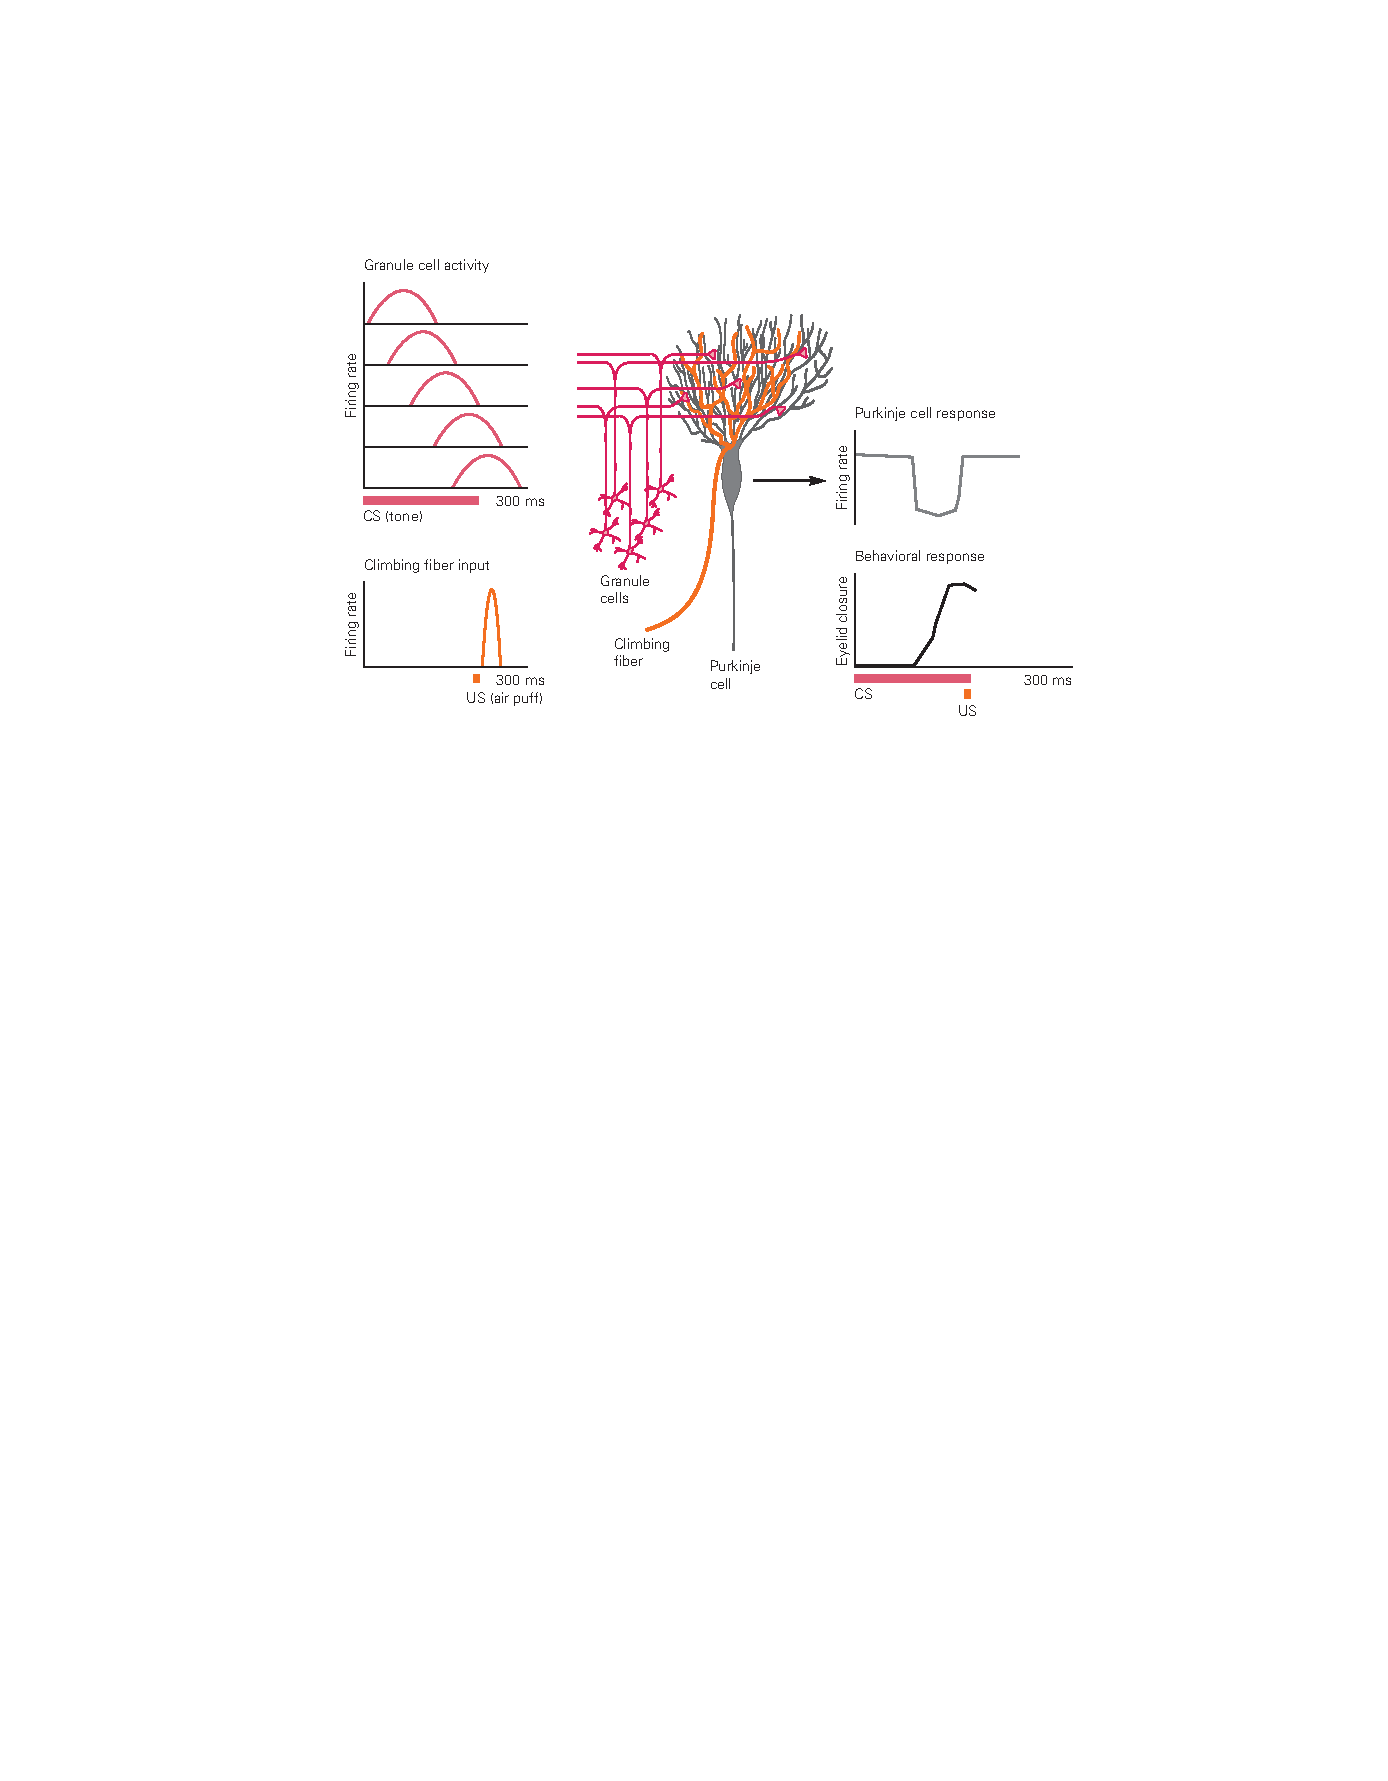
\includegraphics[width=0.92\linewidth]{chap05/fig_5_8}
	\caption{小脑在眨眼条件反射中的假设作用。
		有关\textit{条件刺激}和\textit{非条件刺激}的信息分别通过苔藓和攀爬纤维通路传递。
		在\textit{非条件刺激}呈现之前活跃的颗粒细胞突触被攀爬纤维输入引起的长期抑制逐渐减弱。
		这有助于浦肯野细胞激活的暂停,恰好在\textit{非条件刺激}之前发生。
		由于浦肯野细胞是抑制性的,这种暂停会激发小脑核和红核中的下游神经元,从而驱动眼睑闭合。}
	\label{fig:5_8}
\end{figure}


了解小脑如何介导学习的关键是发现复杂的尖峰触发颗粒细胞和浦肯野细胞之间突触的可塑性。
具体来说,来自突触前颗粒细胞的输入与突触后浦肯野细胞中的复杂尖峰同时出现,导致颗粒细胞输入持续减弱,这是一种称为小脑长期抑制的可塑性形式(图~\ref{fig:5_8})。
因此,对于\textit{非条件刺激}的每次出现,在\textit{非条件刺激}之前立即激活的颗粒-浦肯野细胞突触的强度都会降低。
由于在\textit{非条件刺激}预期到达时间之前颗粒细胞兴奋减少,这种可塑性导致浦肯野细胞放电中逐渐出现学习性暂停。


浦肯野细胞放电的减少如何导致习得性运动反应?
浦肯野细胞通常是自发活跃的,它们会抑制下游靶点。 
小脑区域的浦肯野细胞接收与眼睛有害刺激相关的攀爬纤维输入,与神经元形成突触,间接激活产生眼睑闭合的肌肉。
因此,习得的浦肯野细胞放电暂停导致眼睑在正确的时刻闭合以保护眼睛。
适当的暂停时间被认为是由颗粒细胞中多种时间反应模式介导的。
计算机仿真表明,如果单个颗粒细胞在\textit{条件刺激}后的不同延迟处活跃或表现出锁定到\textit{条件刺激}的各种不同但可重复的时间模式,则可以通过颗粒-浦肯野细胞突触的可塑性来解释适当定时响应的学习。


由于技术挑战,对于参与眨眼调节的哺乳动物小脑区域的颗粒细胞,尚未获得此类时间表征的直接证据。
然而,在类似于鱼类小脑的结构中的颗粒细胞中观察到了多种时间模式。
更广泛地说,对小脑的研究,包括对眨眼条件反射的研究,提供了一个具体的例子,说明神经回路如何通过反复试验来调节学习,甚至是学习更复杂的运动技能,如演奏乐器。
浦肯野细胞整合了与动物的外部世界和内部状态相关的丰富多样的信号(由颗粒细胞传递),以及关于错误或意外事件的高度特异性信息(由攀爬纤维传递)。
攀爬纤维起到老师的作用,削弱了之前活跃的突触,因此可能导致错误。
突触强度的这些变化改变了浦肯野细胞的放电模式,并凭借特定的布线模式改变了行为,从而逐渐减少了错误。


小脑和大脑皮层,包括海马区,是关于学习和记忆的大量实验和理论研究的焦点。 
技术进步开辟了研究突触动作、单个细胞和回路对记忆相关现象的贡献的新方法。



\section{亮点}

1. 神经编码描述了神经元活动如何表示刺激的特征或预期的动作。
解码是指解释神经活动以揭示编码信号的逆过程。
神经反应的数学解码可用于解释神经回路执行的计算并驱动假肢装置。 


2. 神经回路高度相互关联,但使用了一些基本主题来表征它们的功能和操作模式。 
前馈回路处理信息以从感觉流中提取结构和意义。 
循环回路可以执行时间处理并生成动态活动以驱动运动响应。


3. 大多数神经元接受兴奋性和抑制性输入的微调平衡。 
这种平衡响应感官刺激的微小变化可以唤起动作电位输出。


4. 神经活动的水平必须经常保持很多秒。 
循环激发网络提供了一种机制来产生神经输出的持久变化。


5. 突触可塑性支持构成学习和记忆基础的神经回路的更持久变化。
赫布可塑性可以从一组复杂的输入中提取有趣的信号,而无需监督(“老师”)。
小脑皮层的突触可塑性由\textit{误差信号}(一种监督形式)驱动,用于调整运动反应和学习时间关系。



